\section{Erasure Coded Storage} \label{sec:ec}
In the following two cases are investigated; Case A where the lead node performs the encoding and Case B where the lead node delegates to another node to perform the encoding.\\
For both cases systematic Reed-Solomon error correction is used, where the data parts are directly saved with a variable amount of parity. The data is always separated into four parts, for the direct data part. To tolerated one node failure, parity is 50\% overhead (i.e. 2 blocks) and for two node failures, parity is 200\% (i.e. 8 blocks). This is illustrated in figure \ref{fig:rs_sys}. These cases are illustrated in figure \ref{fig:ecs}.\\ 
The time to encode and store, can be defined by the number of tolerated node failures $l$, the data rate $R$, the size of the file in bits $s$, computation time $T_{process}$, and the time to encode $R_{enc}$ and decode $R_{dec}$.

\begin{figure}[H]
	\centering
	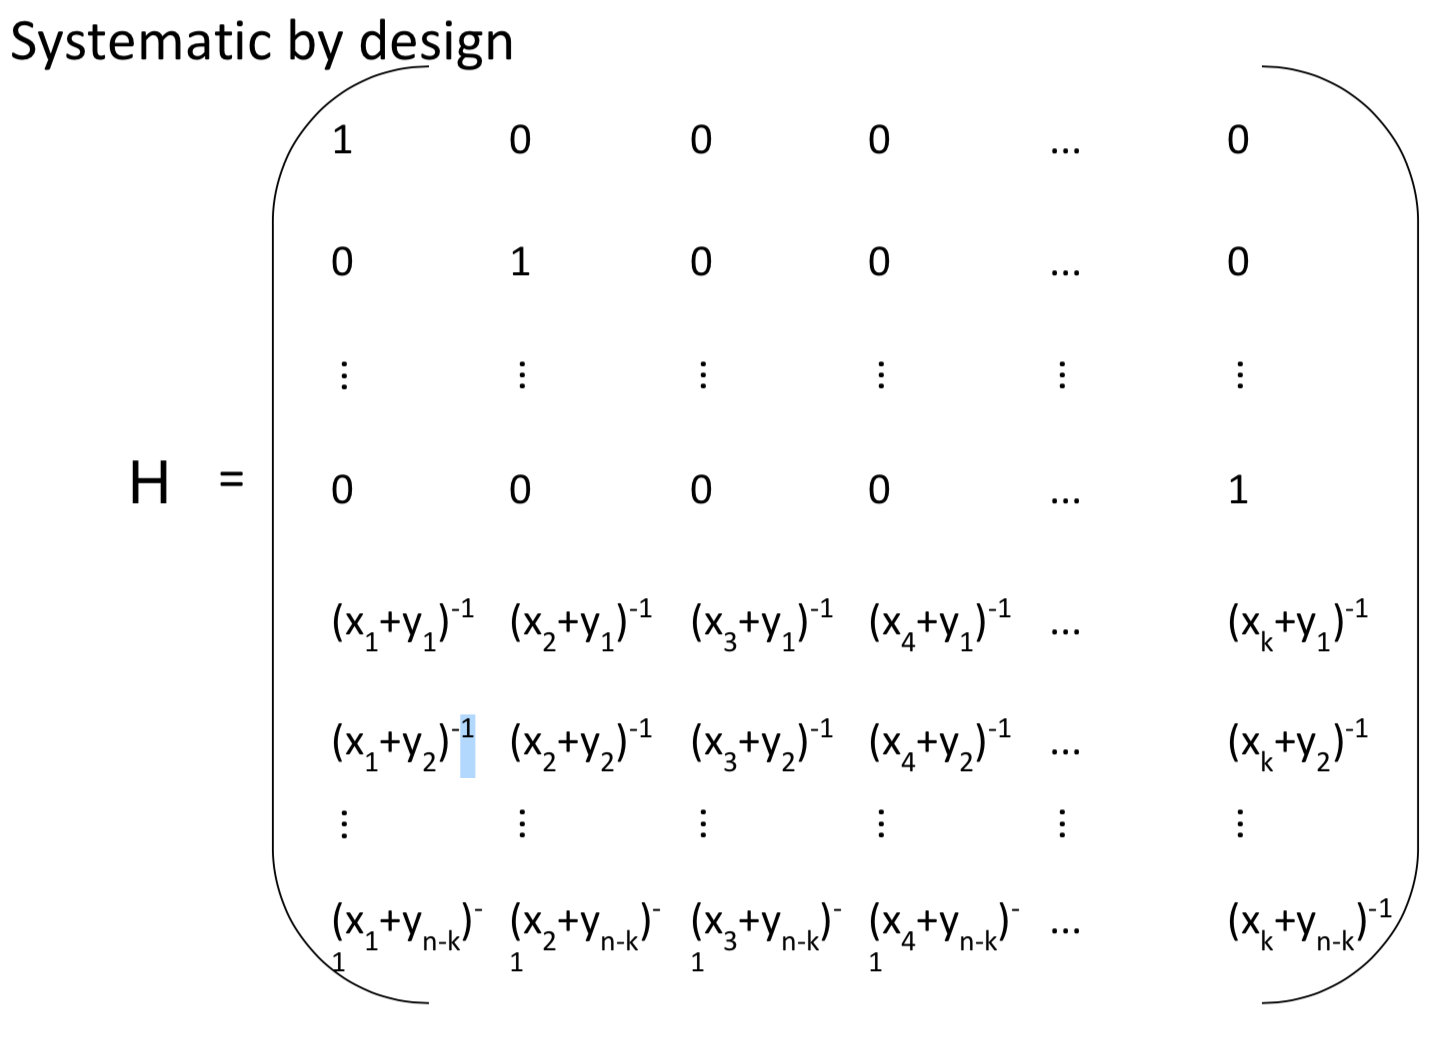
\includegraphics[width=0.6\textwidth]{figures/rs_sys}
	\caption{Systematic Reed-Solomon}
	\label{fig:rs_sys}
\end{figure}

\begin{figure}[H]
    \centering
    \begin{subfigure}{.35\textwidth}
        %\centering
        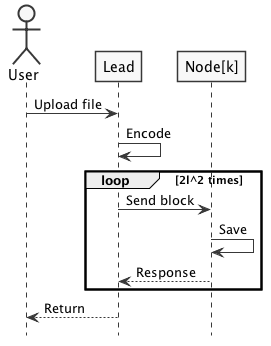
\includegraphics[width=\textwidth]{figures/e3a.png}
        \caption{Case A}
    \end{subfigure}
    \hspace{30px}
    \begin{subfigure}{.42\textwidth}
        %\centering
        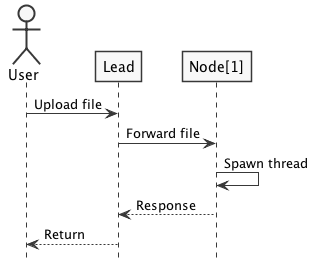
\includegraphics[width=\textwidth]{figures/e3b.png}
        \caption{Case B}
    \end{subfigure}
    \caption{Erasure Code Strategy}
    \label{fig:ecs}
\end{figure}

\subsubsection*{Time to generate redundancy}
\textit{Case A:} 
\begin{align}
    T_{gen} = R \cdot s + R_{enc} \cdot s + 2l^{2} \cdot R \cdot block\_size + T_{process}
\end{align}
\textit{Case B:} 
\begin{align}
    T_{gen} = 2R \cdot s + R_{enc} \cdot s + 2l^{2} \cdot R \cdot block\_size \cdot \frac{2}{3} + T_{process}
\end{align}

\subsubsection*{Time for lead node to finish}
\textit{Case A:} 
\begin{align}
    T_{lead} = R \cdot s + R_{enc} \cdot s + 2l^{2} \cdot R \cdot block\_size + T_{process}
\end{align}
\textit{Case B:} 
\begin{align}
    T_{lead} = 2R \cdot s + T_{process}
\end{align}

\subsubsection*{Access time}
\begin{align}
    T_{access} = 2l^{2} \cdot R \cdot block\_size + R_{dec} \cdot s + R \cdot s + T_{process}
\end{align}

\subsubsection*{Measurements}
\begin{table}[H]
    \begin{tabularx}{\textwidth}{|X|X|X|X|X|}
        \hline
        \cellcolor{lightgray}\textbf{Size} & \cellcolor{lightgray}\textbf{Time Case A [s] (l=1)} & \cellcolor{lightgray}\textbf{Time Case A [s] (l=2)} & \cellcolor{lightgray}\textbf{Time Case B [s] (l=1)} & \cellcolor{lightgray}\textbf{Time Case B [s] (l=2)} \\\hline
        10KB  & 0.25   & 0.43   & 0.06   & 0.06   \\\hline
        100KB & 0.37   & 0.79   & 0.18   & 0.18   \\\hline
        1MB   & 1.49   & 2.73   & 1.09   & 1.13   \\\hline
        10MB  & 13.76  & 22.50  & 11.50  & 11.21  \\\hline
        100MB & 124.26 & 212.74 & 112.17 & 120.30 \\\hline
    \end{tabularx}
    \caption{Measurements, part 1}
	\label{tab:e3meas1}
\end{table}

\begin{table}[H]
    \begin{tabularx}{\textwidth}{|X|X|X|X|X|X|X|}
        \hline
        \cellcolor{lightgray}\textbf{Size} & \cellcolor{lightgray}\textbf{Time Encode [s] (l=1)} & \cellcolor{lightgray}\textbf{Time Encode [s] (l=2)} & \cellcolor{lightgray}\textbf{Time Decode [s] (l=1)} & \cellcolor{lightgray}\textbf{Time Decode [s] (l=2)} & \cellcolor{lightgray}\textbf{Time Download [s] (l=1)} & \cellcolor{lightgray}\textbf{Time Download [s] (l=2)} \\\hline
        10KB  & 0.0014 & 0.0014 & 0.0009 & 0.0009 & 0.14  & 0.14  \\\hline
        100KB & 0.0042 & 0.0067 & 0.0019 & 0.0030 & 0.27  & 0.28  \\\hline
        1MB   & 0.0260 & 0.0751 & 0.0207 & 0.0264 & 0.59  & 0.57  \\\hline
        10MB  & 0.3045 & 0.8796 & 0.1612 & 0.2829 & 4.83  & 4.61  \\\hline
        100MB & 2.9528 & 8.8063 & 1.4422 & 2.1291 & 42.94 & 39.80 \\\hline
    \end{tabularx}
    \caption{Measurements, part 2}
	\label{tab:e3meas2}
\end{table}

Differences in Case A, with different l. Higher l takes longer time, as the lead has to encode and distribute more blocks i.e. more overhead is introduces. \\
Differences in Case B, with different l. Makes no difference, as the lead node, always have to send the raw file once. \\
Differences between Case A and Case B. Case A takes longer time for the lead node to be freed, since it has to do the encoding and sending the overhead.
Encode variance with different l. Takes slightly longer with higher l, as more encoded blocks have to be generated, especially with bigger files\\
Decode variance with different l. Takes slightly longer with higher l, as the data is more encoded. Bigger files also takes longer \\
Download with different l. Makes no difference as the same amount of blocks have to fetched from nodes (i.e. 4) and since the decode time is nearly negligible compared to the transport time.